\chapter{Completeness analysis}
\label{chapter:cad}


\begin{table}
\caption{ \textbf{To be updated.} \smr\ Level1B and Level2 data count by frequency mode.
Level2 data are further categorized into two classes: "All-Level2" and "Ok-Level2",
where "Ok-Level2" means that the Level2 processing produced a result with a valid
quality.
Column "succes rate - Level2" and "succes rate - Ok Level2" describes the fraction of
"Level2 count - All" over "Level1B count" and "Level2 count - ok" over "Level2 count - All".}
\label{table:count}
\scalebox{0.965}{%
\begin{tabular}{| *{6}{c|} }
    \hline
\textbf{Frequency mode} & \textbf{Level1B count}
            & \multicolumn{2}{c|}{\textbf{Level2 count}}
                    & \multicolumn{2}{c|}{\textbf{Succes rate [\(\%\)]}} \\
    &    & All & Ok & Level2 & Ok Level2  \\
    \hline
    \hline
  01 & 1924043 & 1711616 & 1494160 & 89.0 & 87.3\\
  \hline
  02 & 1907511 & 1541197 & 1463753 & 80.8 & 95.0\\
  \hline
  08 & 400901 & 335727 & 329448 & 83.7 & 98.1\\
  \hline
  13 & 359696 & 294299 & 269568  & 81.8 & 91.6\\
  \hline
  14 & 365195 & 218611 & 201758 & 59.9 & 92.2\\
  \hline
  19 & 400037 & 332057 & 235699 & 83.0 & 71.0\\
  \hline
  21 & 344476 & 299992 & 276128 & 87.1 & 92.0\\
  \hline
  22 & 93374 & 56768 & 56452 & 60.8 & 99.4\\
  \hline
  24 & 15794 & 12873 & 12655 & 81.5 & 98.3\\
  \hline
\end{tabular}}
\end{table}


Table~\ref{table:count} and Figure~\ref{fig:l2cad-fm1} to
Figure~\ref{fig:l2cad-fm24} show the amount af available Level1B
data and succesfully processed Level2 data for the considered
FreqModes by month, from the start of the mission until the
end of 2019. 

The amount of available Level1B data varies during mission,
and there are a number of reasons for this.
During the first six years of the mission \smr\ was operated
both in aeronomy and astronomy mode, and hence less
aeronomy observations are available for these years
compared to after 2008.  
During the most recent years \smr\ has both partly and completely
been turned off during the summer months.
\smr\ is a flexible instrument, as described in Sect.~\ref{sec:odin}
but, in prinicipal, only two frequency modes (FreqModes)
can be applied at a given time. The observation program, or how
often the various FreqModes are used, has been varied during the
mission.

No Level2 data are available after 2019-08-31, as 
ERA-Interim reanalysis data (Level2 processor source for
required altitude, pressure, and temperature data)
were stopped being produced by then.

FreqMode 1 and 2 are the most frequently applied modes, and
about 5000-10000 scans have been observed each month. Level2 processing
generated in a result for the majority (89 and 81\,\%, respectively) of
the available Level1B data. One of the main reason for the
Level2 processing to not generate in a result
is here that some scans do not cover a required
altitude range, or that to few spectra are available within this range,
i.e. not enough spread of the tangent altitude of individual spectra. 
The majority of FreqMode 2 Level2 data have a valid quality.
A valid quality means here that the 
\begin{itemize}

  \item MinLmFactor \([-]\): The minimum value of the Levenberg - Marquardt factor during the OEM iterations, and the

  \item Residual \([K]\):  The difference between the spectra matching retrieved state and
   used measurement spectra

\end{itemize}
are below specified thresholds (2 and 1.5\,K, respectively).
This is also true for FreqMode 1, except for data after summer
of 2014 where a large fraction of the produced Level2 data
have an unsatisfactory quality. Instrumental problems
with this mode for the later part of the mission is discussed
in \cite{dds}.

Level2 processing generated in a result for about 84\,\%
of the FreqMode 8 observations. The fraction of valid Level2
data is high (98 \,\%) for FreqMode 8.
One reason for this high fraction of valid Level2 data
is that the quality criteria is less strict for FreqMode 8,
compared to most other modes (except 13 and 19).
These mode showed considerable sideband leakage, and a correction
has been applied ~\cite{dds}. 


% 
% A possible reason for this is that this mode showed considerable
% sideband leakage, and a correction has been applied ~\cite{dds},
% but the result seems to be that this results in Level2 data
% that are not classified as valid. \textbf{TODO: check if our
% current quality filter is to hard, or if this is the truth.}

For the water vapor modes around 557 GHz (FreqMode
13 and 19) the Level2 processing generates in a result for
about 82\,\% of the scans. The fraction of Level2 
data with a valid quality is 92 and 71 \,\% for FreqMode
13 and 19, respectively.
Issues with FreqMode 13 and 19 observations are discussed
in \cite{dds}.
 
Level2 processing of the FreqMode 21 (\chem{NO} mode)
generated in a result for about 87\,\% of the scans.
Most of this data (92\,\%) have a satisfactory quality.

FreqMode 14, 22, 24 are deployed for \chem{CO} observations.
The frontend used for these observations have been unstable
(drifting in frequency), and that can result in that the 
\chem{CO} signature is not covered in observed spectra 
of some of the scans. This gives that the fraction of
level2 data produced is lower for those modes.
However, the data are valid for a high percentage
(above 92\,\%) for the Level2 data actually produced.  
 

\begin{figure}[t]
\centering
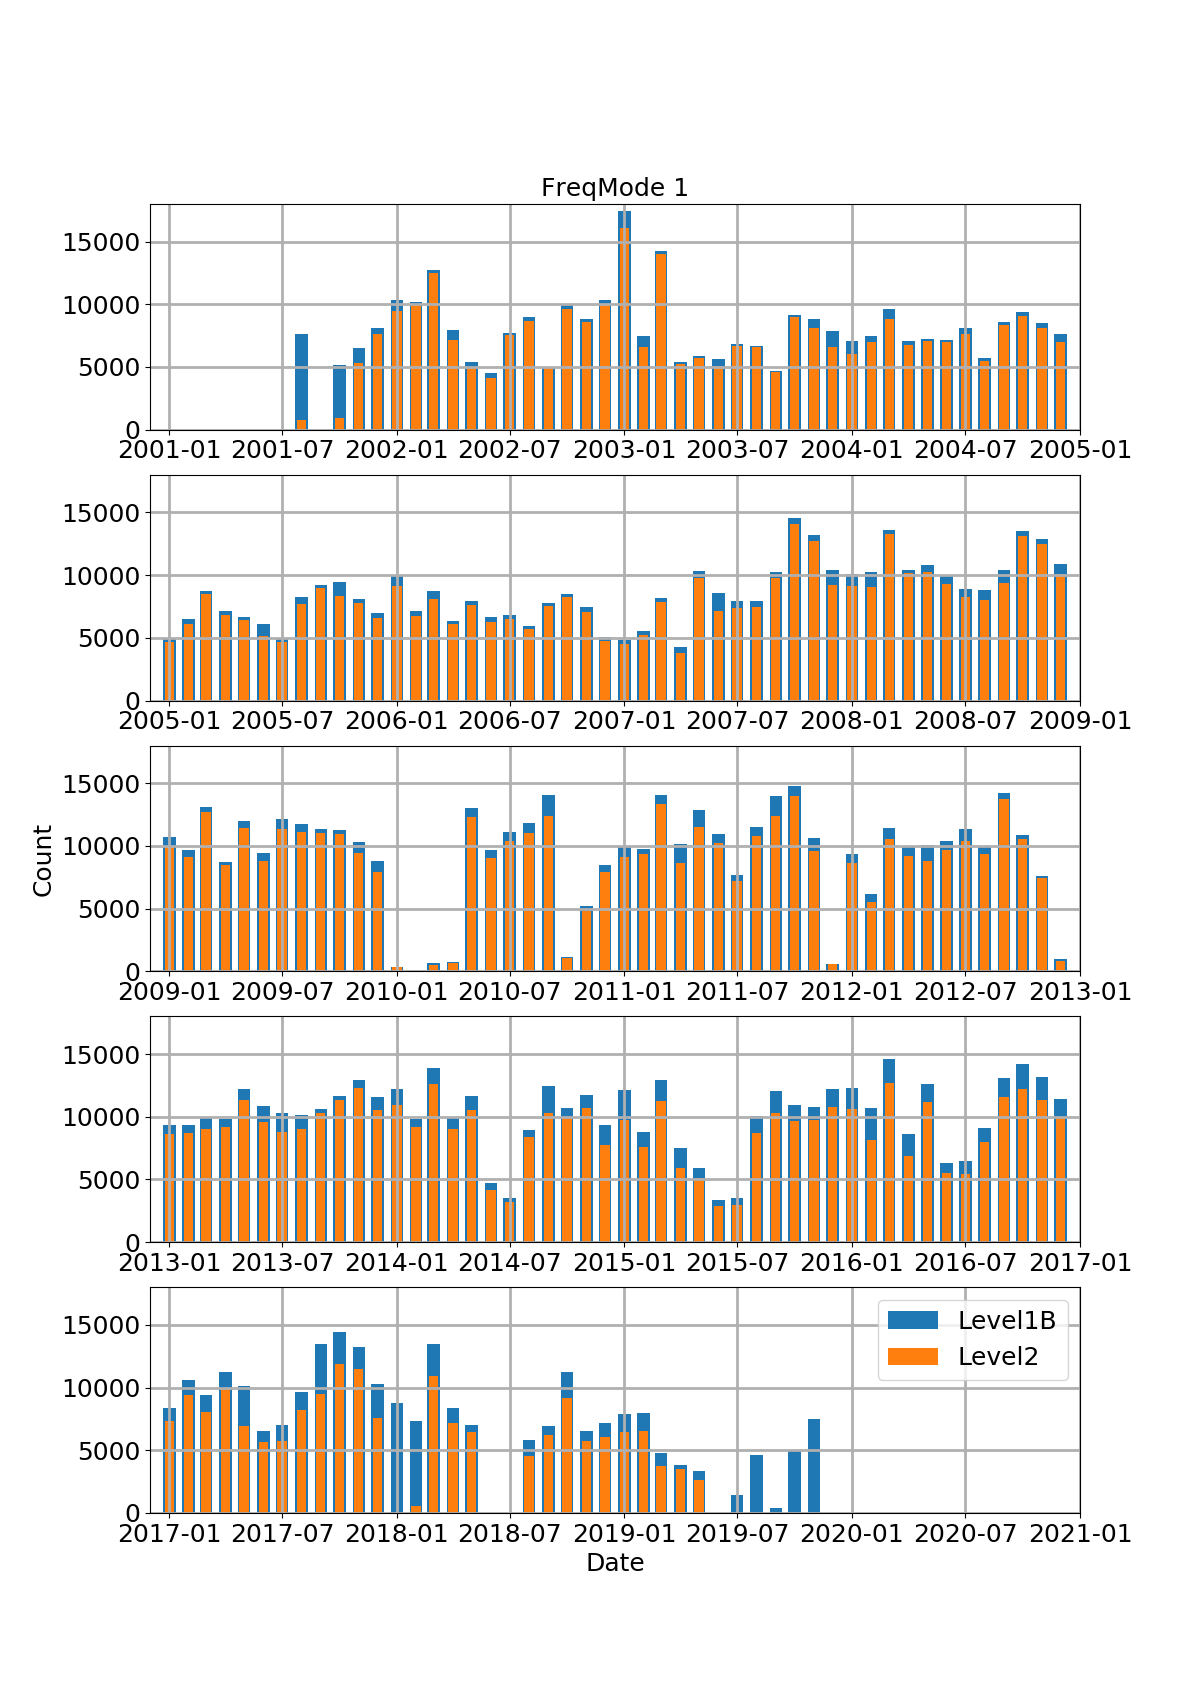
\includegraphics[width=1.0\textwidth]{l2cad-fm1.png}
\caption{Number of available Level1b and succesfully processed Level2
scans by month for FreqMode 1, during the complete \smr\ mission.}
\label{fig:l2cad-fm1}
\end{figure}

\begin{figure}[t]
\centering
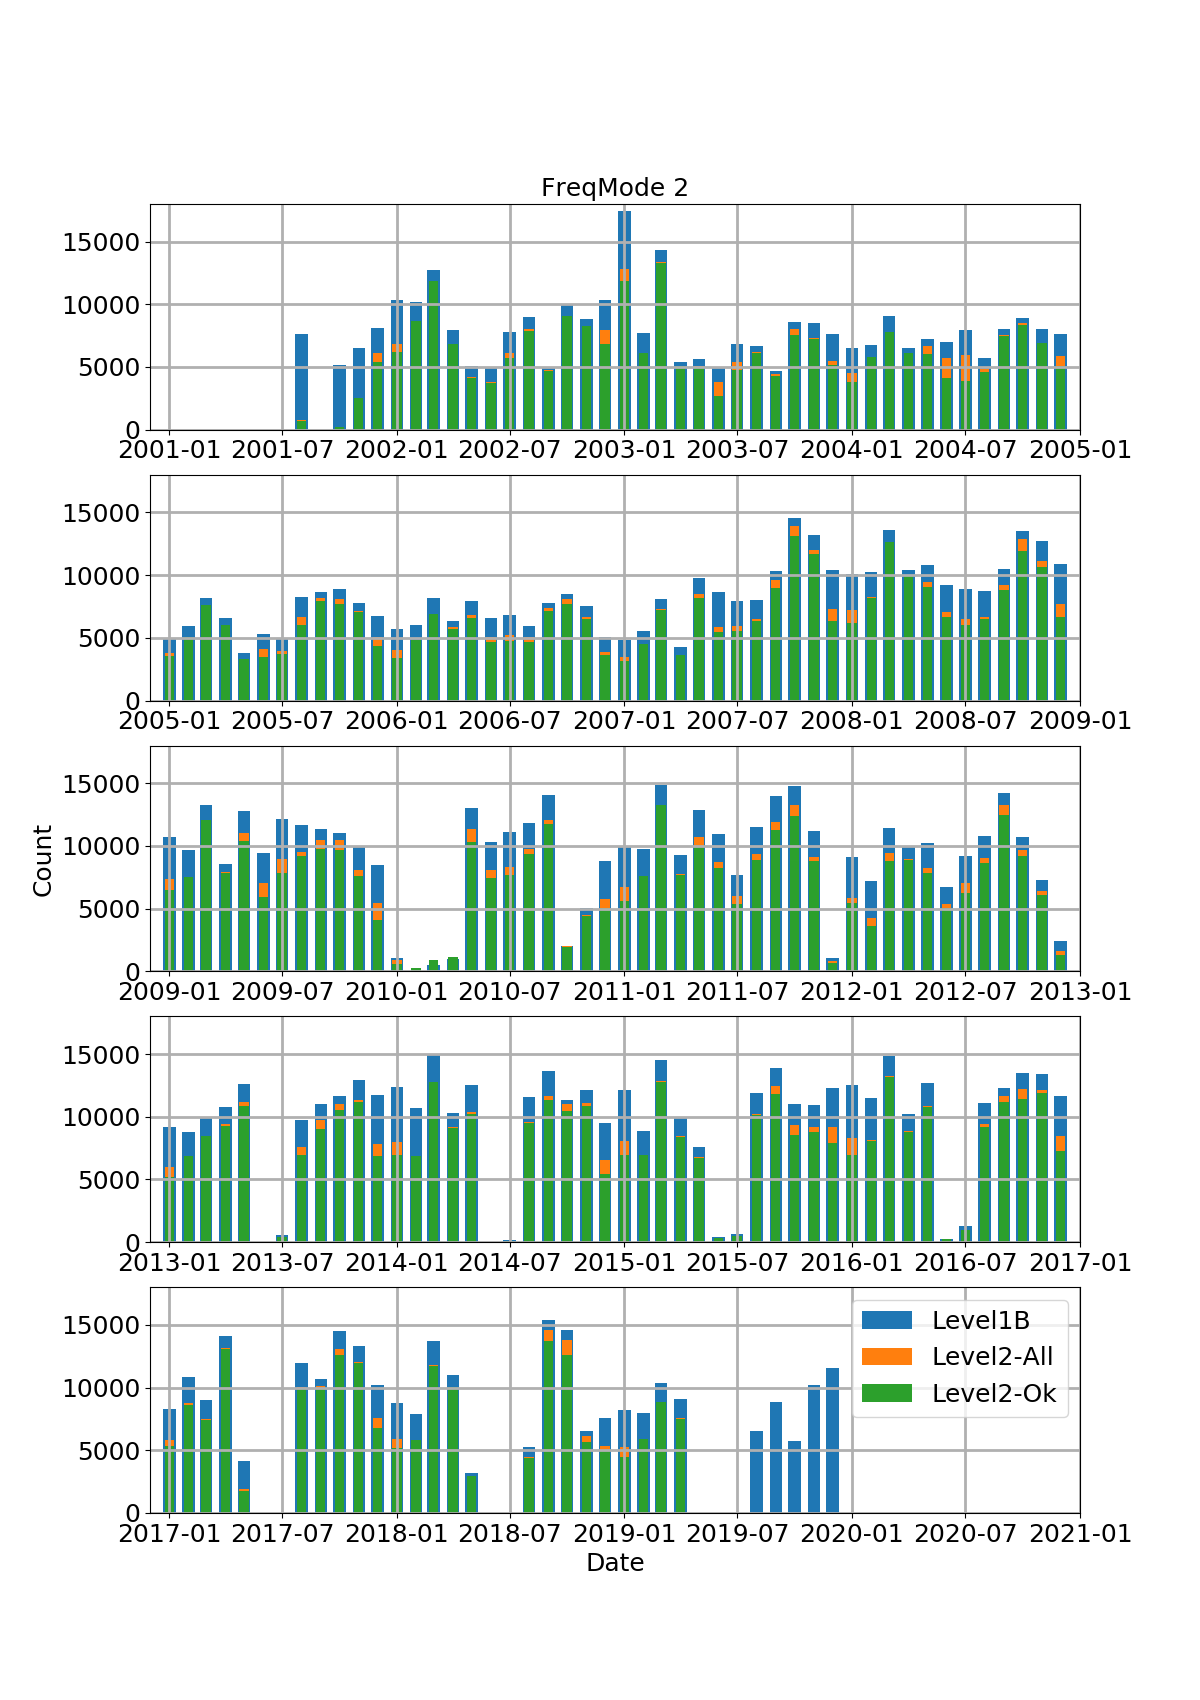
\includegraphics[width=1.0\textwidth]{l2cad-fm2.png}
\caption{As Figure~\ref{fig:l2cad-fm1} but for FreqMode 2.}
\label{fig:l2cad-fm8}
\end{figure}

\begin{figure}[t]
\centering
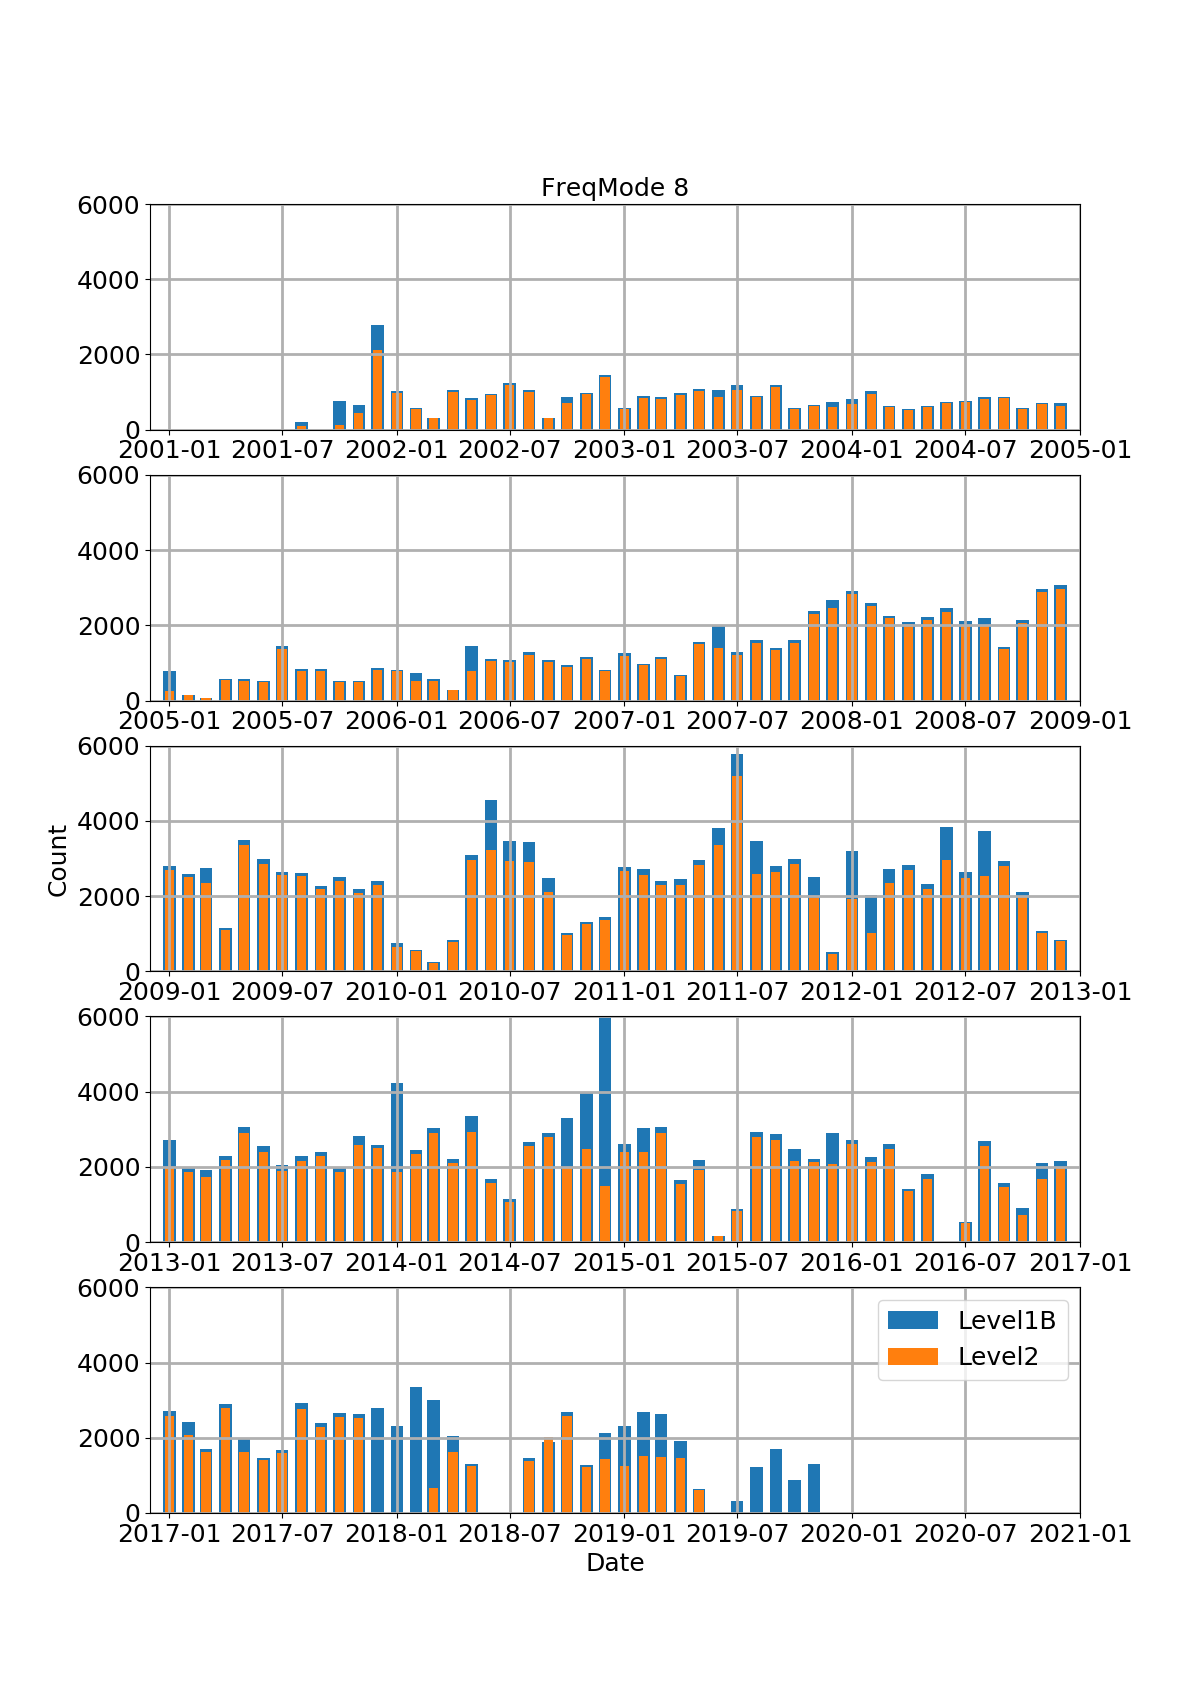
\includegraphics[width=1.0\textwidth]{l2cad-fm8.png}
\caption{As Figure~\ref{fig:l2cad-fm1} but for FreqMode 8.}
\label{fig:l2cad-fm8}
\end{figure}

\begin{figure}[t]
\centering
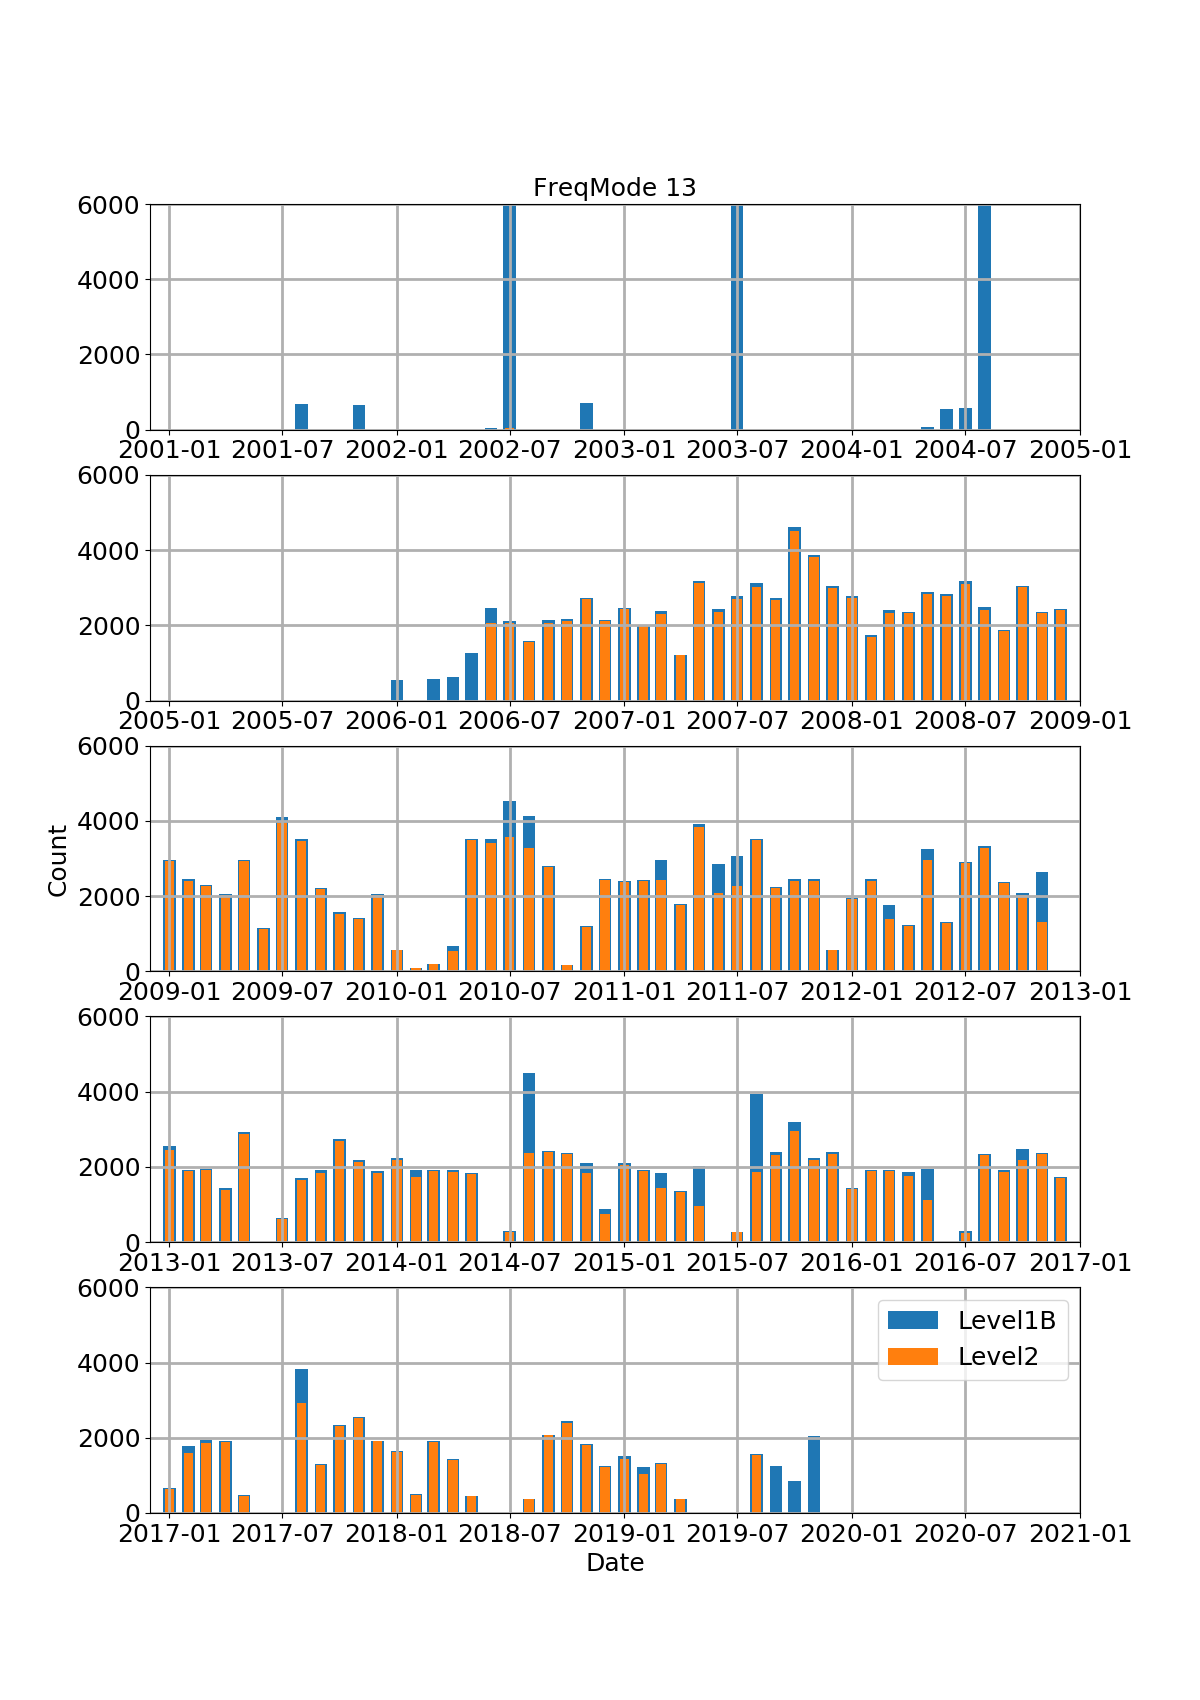
\includegraphics[width=1.0\textwidth]{l2cad-fm13.png}
\caption{As Figure~\ref{fig:l2cad-fm1} but for FreqMode 13.}
\label{fig:l2cad-fm13}
\end{figure}

\begin{figure}[t]
\centering
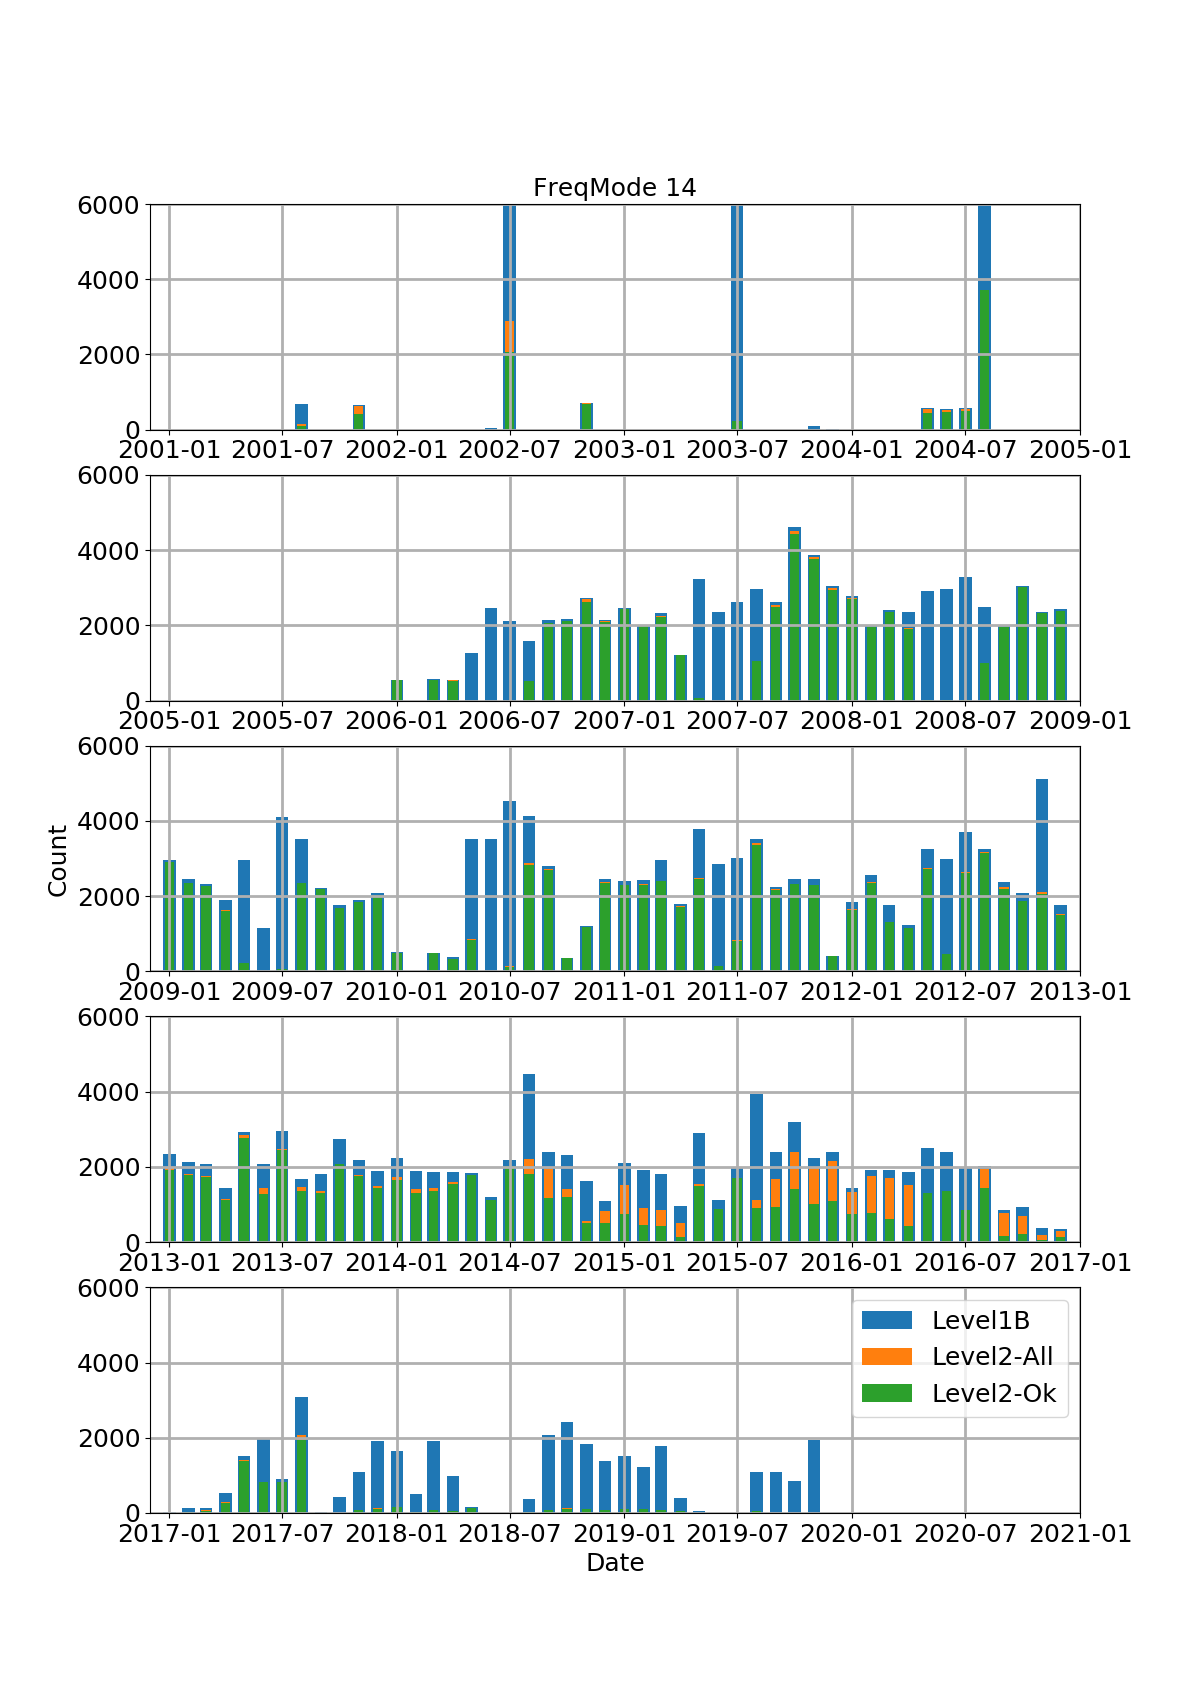
\includegraphics[width=1.0\textwidth]{l2cad-fm14.png}
\caption{As Figure~\ref{fig:l2cad-fm1} but for FreqMode 14.}
\label{fig:l2cad-fm14}
\end{figure}

\begin{figure}[t]
\centering
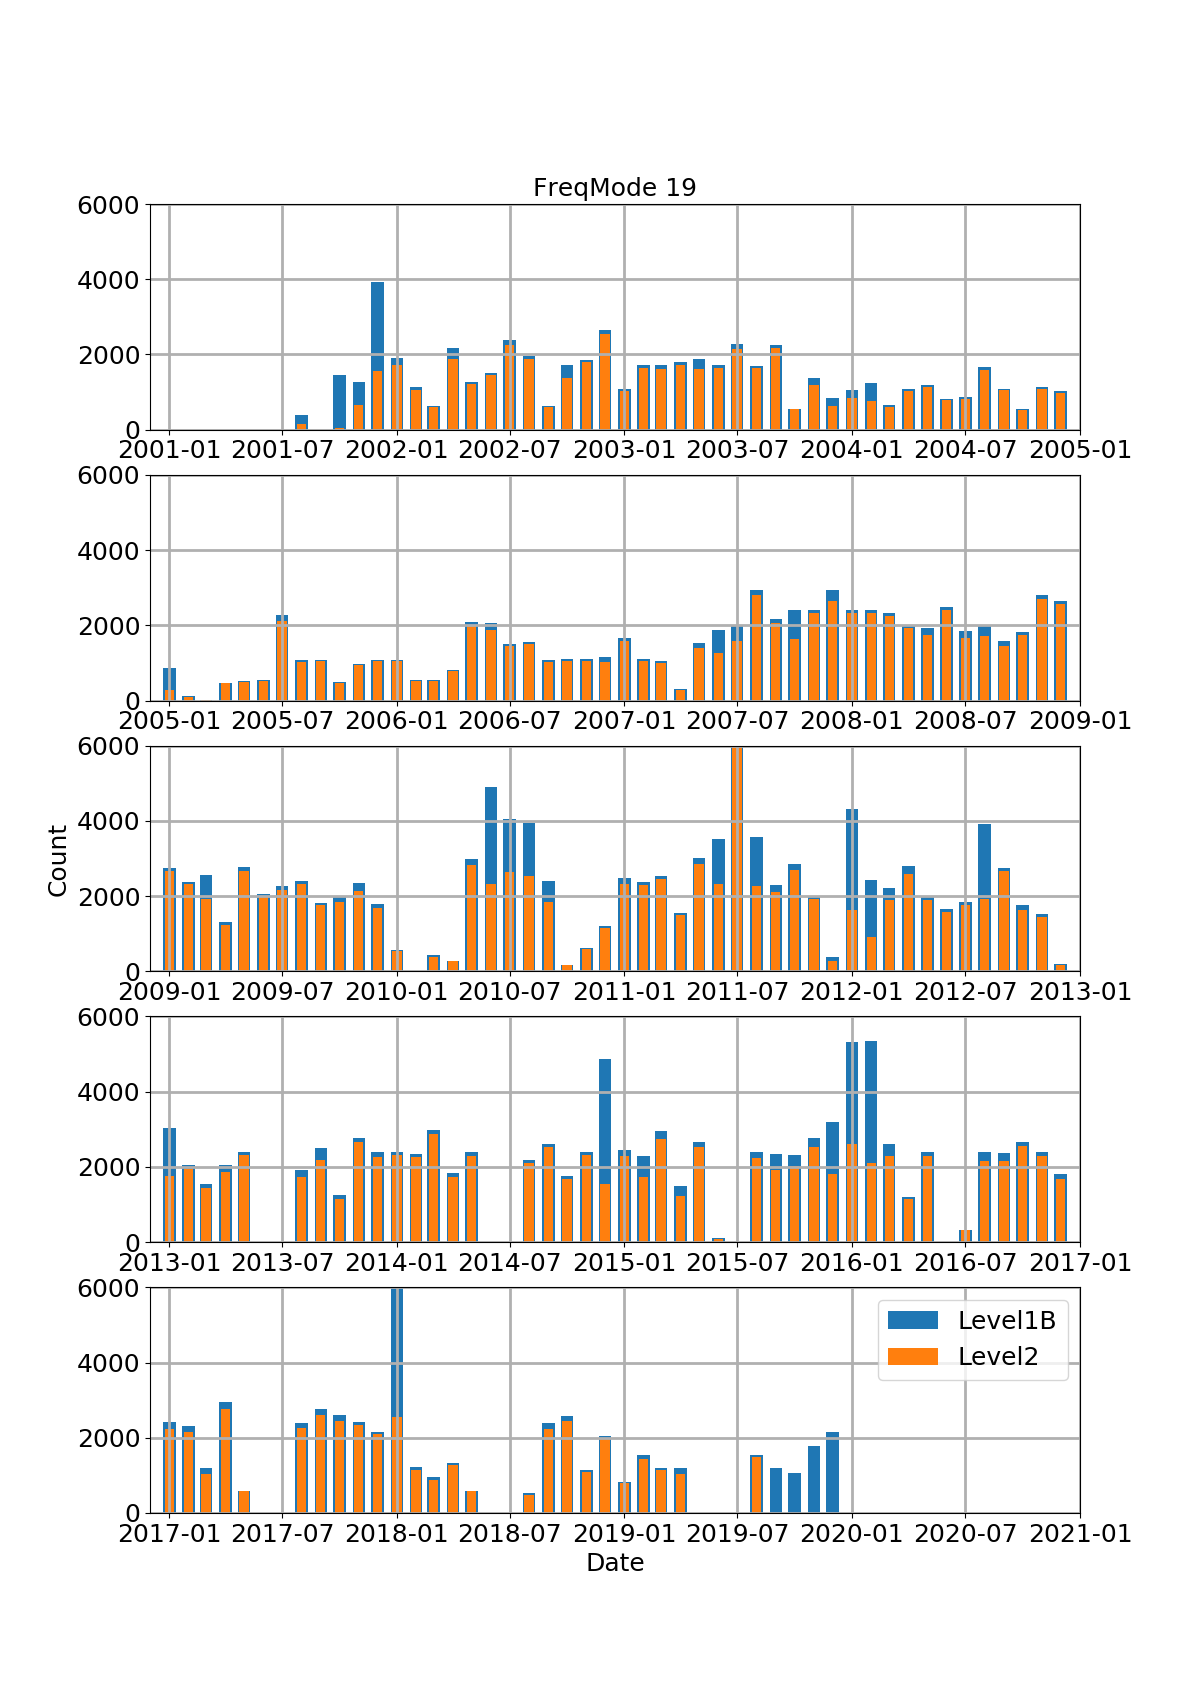
\includegraphics[width=1.0\textwidth]{l2cad-fm19.png}
\caption{As Figure~\ref{fig:l2cad-fm1} but for FreqMode 19.}
\label{fig:l2cad-fm19}
\end{figure}

\begin{figure}[t]
\centering
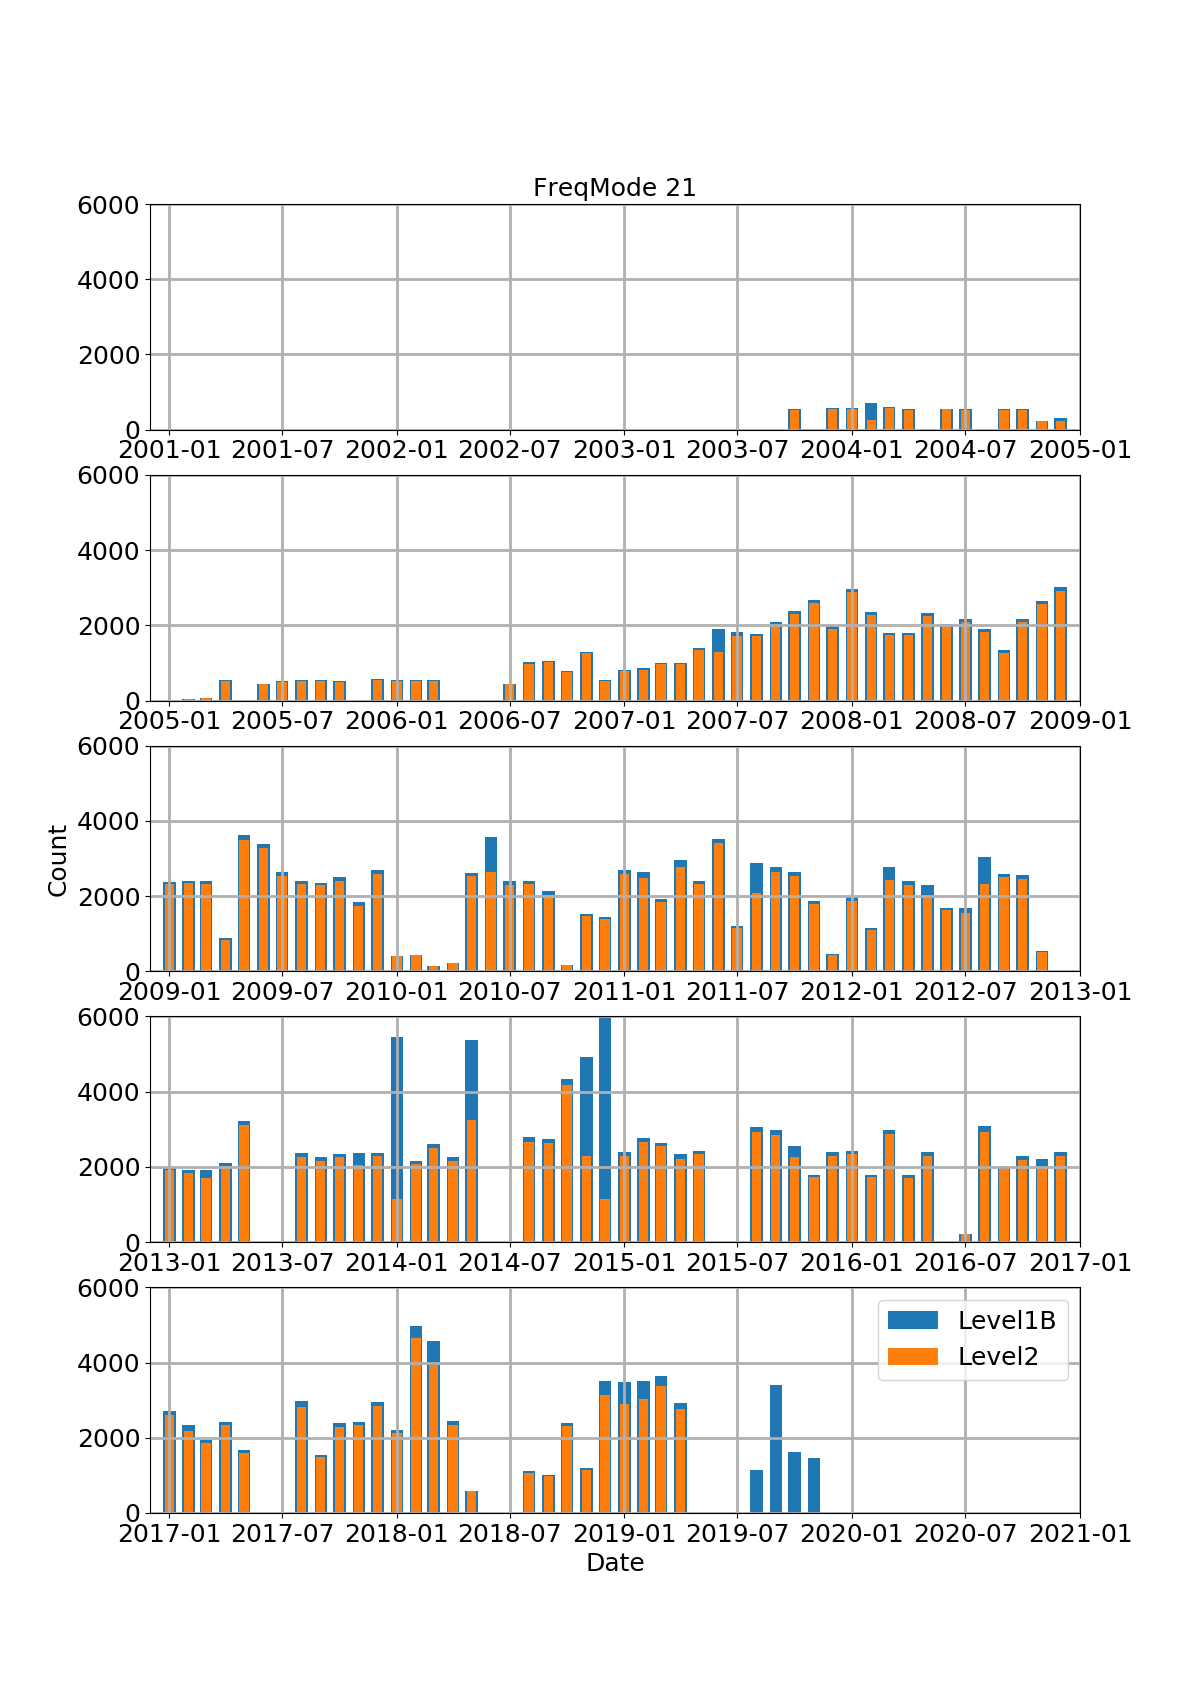
\includegraphics[width=1.0\textwidth]{l2cad-fm21.png}
\caption{As Figure~\ref{fig:l2cad-fm1} but for FreqMode 21.}
\label{fig:l2cad-fm21}
\end{figure}

\begin{figure}[t]
\centering
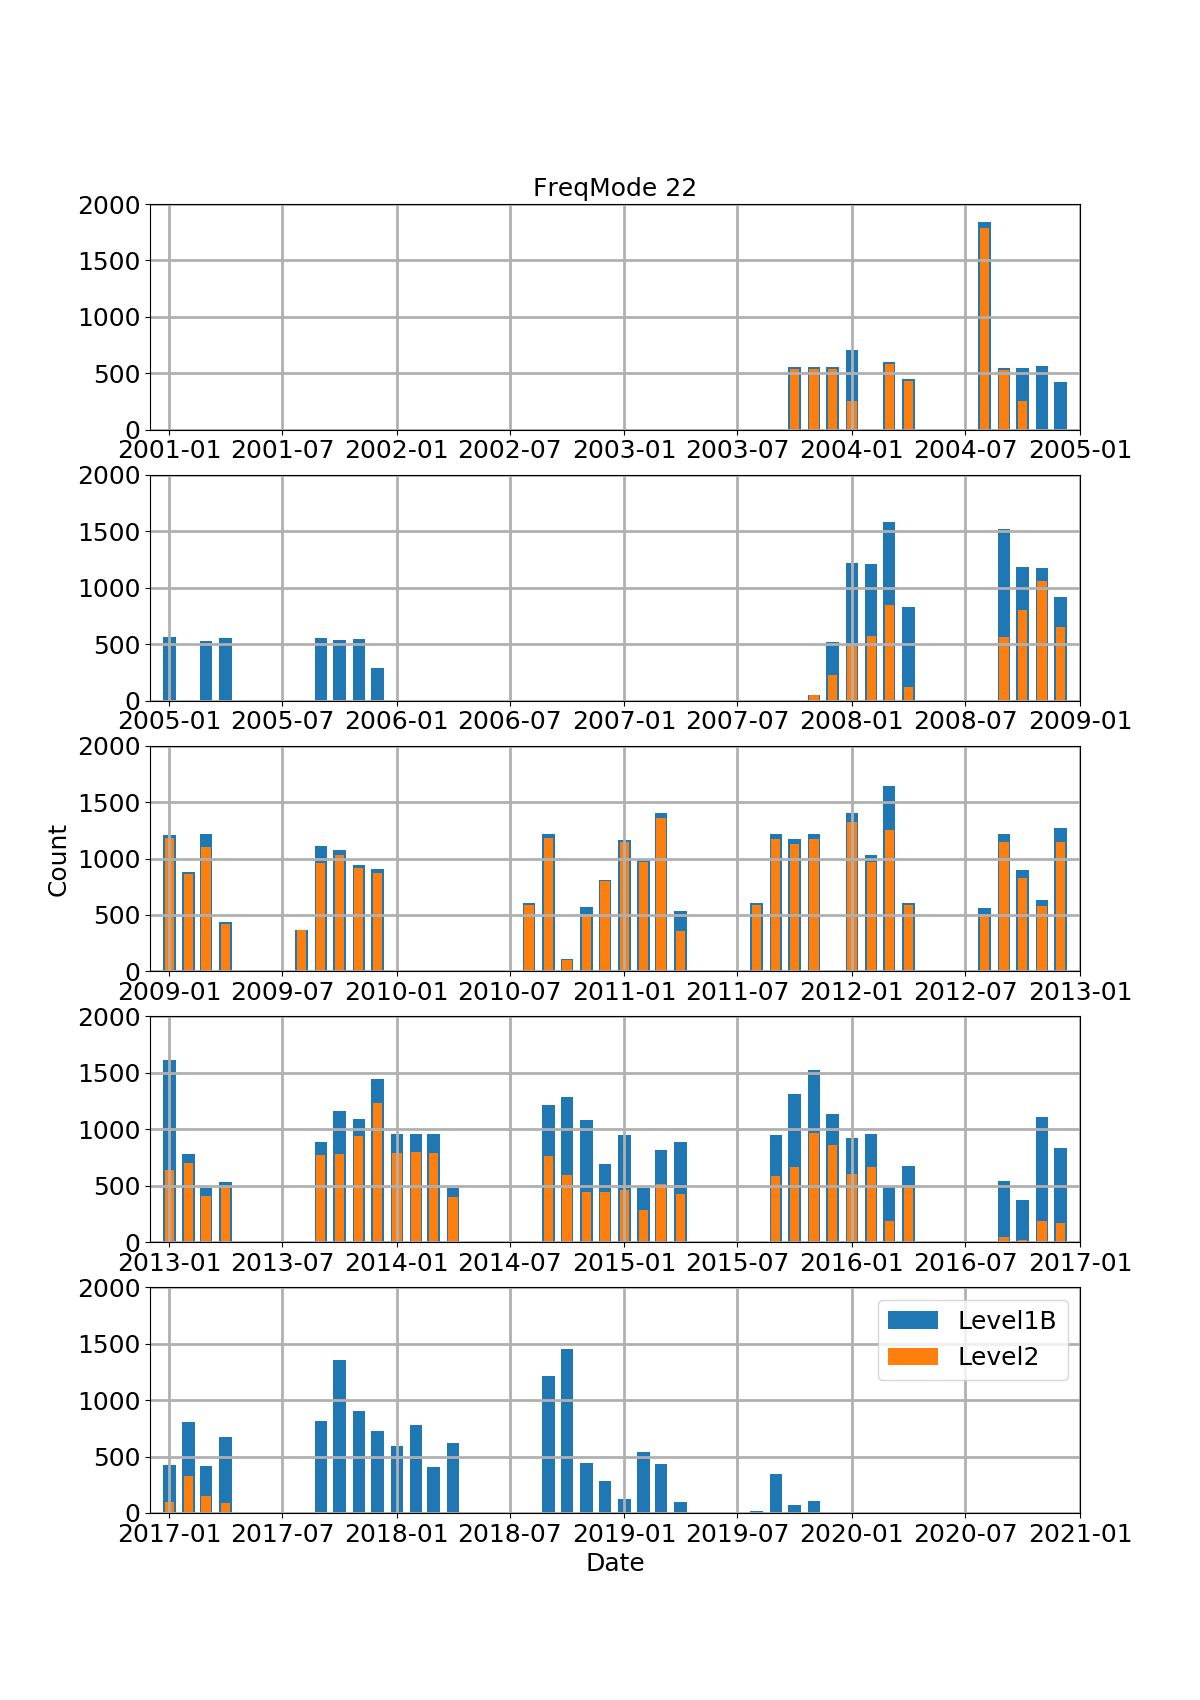
\includegraphics[width=1.0\textwidth]{l2cad-fm22.png}
\caption{As Figure~\ref{fig:l2cad-fm1} but for FreqMode 22.}
\label{fig:l2cad-fm22}
\end{figure}

\begin{figure}[t]
\centering
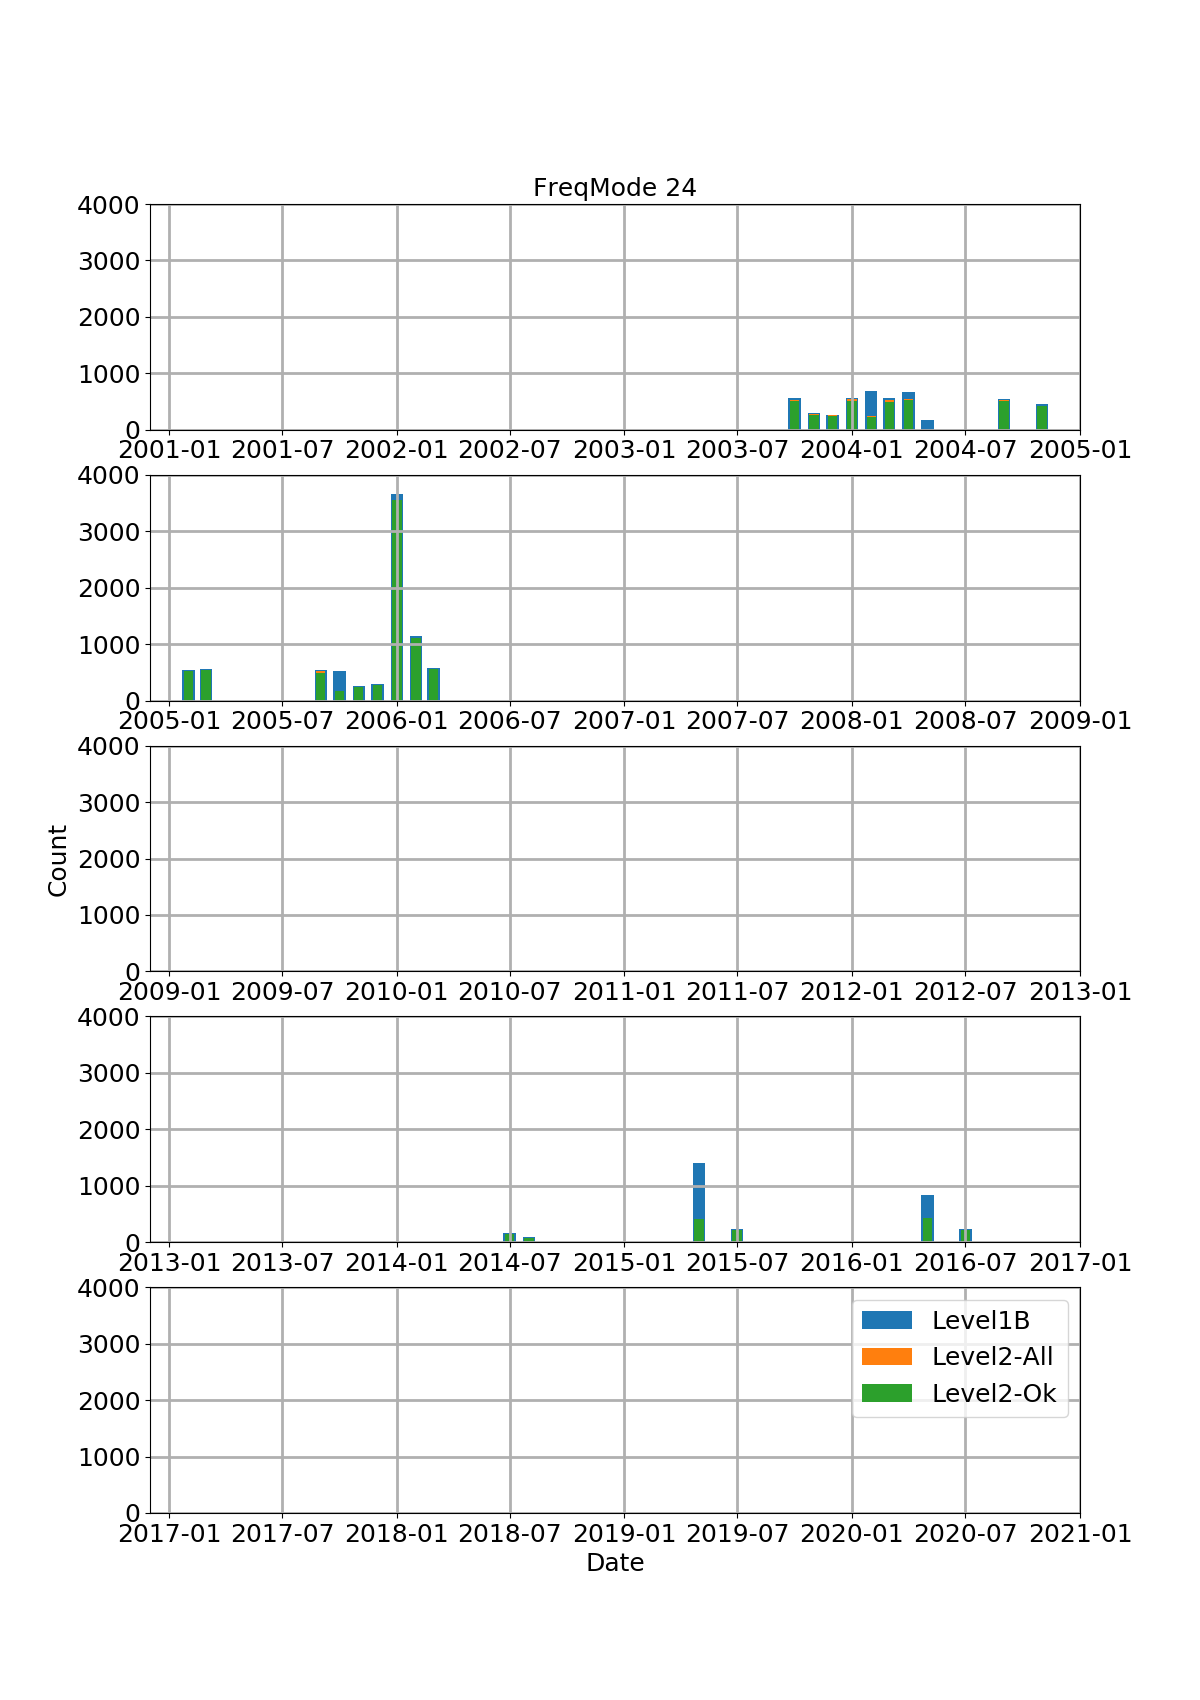
\includegraphics[width=1.0\textwidth]{l2cad-fm24.png}
\caption{As Figure~\ref{fig:l2cad-fm1} but for FreqMode 24.}
\label{fig:l2cad-fm24}
\end{figure}
